\subsubsection{UML Description}
The UML below describes at high-level the model of the system to be developed. It considers the basic service together with the advanced function 1 and advanced function 2 previously specified. The UML does not include every class that will be necessary to define the complete architecture of the system.\\
CLup more functions than basic service. The manager registers to the application with all necessary information and the manager could activate the advance function or advance function 2 at any time. The user who use mobile could simply download the application on his/her device and use it and user who doesn't have mobile could easily go near the shop and get a ticket from ticket machine.\\
Here we can identify the main aspect of CLup:
\begin{itemize}
    \item The user could request to be in line for a shop and application shows estimated waiting time to him/her.
    \item The user could book a visit for a shop. This booking contains the date and time user wants to go shopping besides, user can add the categories of item he/she has in shopping list. The application could suggest the user free slots and user book them.
    \item The application based the current location of users must notify them and ask them to approach the shop in a suitable time.
    \item The application must notify people when it's their turn to go shopping.
    \item At the entrance time, the QR code generated in the app must be scanned to ensure they come in the right time.
    \item At the checkout, the cashier must scan the QR code of user and the system must add shopping information (like duration of shopping, category of item which user buy) to user history.
\end{itemize}

\begin{figure}[H]
  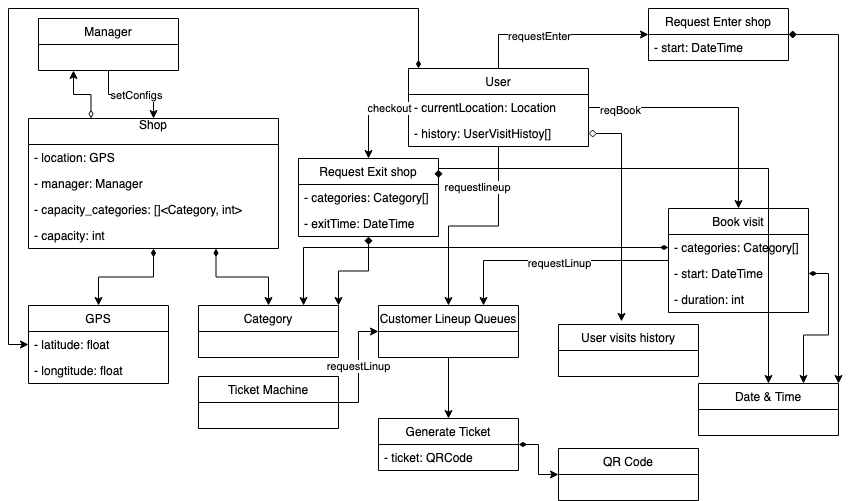
\includegraphics[width=\textwidth,height=\textheight,keepaspectratio]{images/ClassDiagram.png}
  \caption{High level Class Diagram}
\end{figure}